\documentclass[12pt,]{article}
\usepackage{lmodern}
\usepackage{amssymb,amsmath}
\usepackage{ifxetex,ifluatex}
\usepackage{fixltx2e} % provides \textsubscript
\ifnum 0\ifxetex 1\fi\ifluatex 1\fi=0 % if pdftex
  \usepackage[T1]{fontenc}
  \usepackage[utf8]{inputenc}
\else % if luatex or xelatex
  \ifxetex
    \usepackage{mathspec}
  \else
    \usepackage{fontspec}
  \fi
  \defaultfontfeatures{Ligatures=TeX,Scale=MatchLowercase}
    \setmainfont[]{Times New Roman}
\fi
% use upquote if available, for straight quotes in verbatim environments
\IfFileExists{upquote.sty}{\usepackage{upquote}}{}
% use microtype if available
\IfFileExists{microtype.sty}{%
\usepackage{microtype}
\UseMicrotypeSet[protrusion]{basicmath} % disable protrusion for tt fonts
}{}
\usepackage[margin=2.54cm]{geometry}
\usepackage{hyperref}
\hypersetup{unicode=true,
            pdftitle={Examining the Hydrologic Properties of the Missouri River Basin},
            pdfauthor={Rachel Bash, Keqi He, Caroline Watson, and Haoyu Zhang},
            pdfborder={0 0 0},
            breaklinks=true}
\urlstyle{same}  % don't use monospace font for urls
\usepackage{longtable,booktabs}
\usepackage{graphicx,grffile}
\makeatletter
\def\maxwidth{\ifdim\Gin@nat@width>\linewidth\linewidth\else\Gin@nat@width\fi}
\def\maxheight{\ifdim\Gin@nat@height>\textheight\textheight\else\Gin@nat@height\fi}
\makeatother
% Scale images if necessary, so that they will not overflow the page
% margins by default, and it is still possible to overwrite the defaults
% using explicit options in \includegraphics[width, height, ...]{}
\setkeys{Gin}{width=\maxwidth,height=\maxheight,keepaspectratio}
\IfFileExists{parskip.sty}{%
\usepackage{parskip}
}{% else
\setlength{\parindent}{0pt}
\setlength{\parskip}{6pt plus 2pt minus 1pt}
}
\setlength{\emergencystretch}{3em}  % prevent overfull lines
\providecommand{\tightlist}{%
  \setlength{\itemsep}{0pt}\setlength{\parskip}{0pt}}
\setcounter{secnumdepth}{5}
% Redefines (sub)paragraphs to behave more like sections
\ifx\paragraph\undefined\else
\let\oldparagraph\paragraph
\renewcommand{\paragraph}[1]{\oldparagraph{#1}\mbox{}}
\fi
\ifx\subparagraph\undefined\else
\let\oldsubparagraph\subparagraph
\renewcommand{\subparagraph}[1]{\oldsubparagraph{#1}\mbox{}}
\fi

%%% Use protect on footnotes to avoid problems with footnotes in titles
\let\rmarkdownfootnote\footnote%
\def\footnote{\protect\rmarkdownfootnote}

%%% Change title format to be more compact
\usepackage{titling}

% Create subtitle command for use in maketitle
\providecommand{\subtitle}[1]{
  \posttitle{
    \begin{center}\large#1\end{center}
    }
}

\setlength{\droptitle}{-2em}

  \title{Examining the Hydrologic Properties of the Missouri River Basin}
    \pretitle{\vspace{\droptitle}\centering\huge}
  \posttitle{\par}
  \subtitle{\url{https://github.com/cwatson1013/Hydrologic_Data_Analysis_Final_Proj}}
  \author{Rachel Bash, Keqi He, Caroline Watson, and Haoyu Zhang}
    \preauthor{\centering\large\emph}
  \postauthor{\par}
    \date{}
    \predate{}\postdate{}
  
\usepackage{booktabs}
\usepackage{longtable}
\usepackage{array}
\usepackage{multirow}
\usepackage{wrapfig}
\usepackage{float}
\usepackage{colortbl}
\usepackage{pdflscape}
\usepackage{tabu}
\usepackage{threeparttable}
\usepackage{threeparttablex}
\usepackage[normalem]{ulem}
\usepackage{makecell}
\usepackage{xcolor}

\usepackage{float}

\begin{document}
\maketitle

\newpage

\hypertarget{rationale-and-research-questions}{%
\section{Rationale and Research
Questions}\label{rationale-and-research-questions}}

The Missouri River is the largest river in North America (2,540 miles)
and has the second largest watershed (529,000 mi\textsuperscript{2}/339
acres, U.S.-Canada, (Kammerer 1990)). Its watershed covers portions of
ten states, which account for approximately one-sixth of the continental
United States, as well as a small part of Canada (Engineers Missouri
River Basin Water Management Division 2018). The headwater is located in
the Bitterroot Mountains River of northwestern Wyoming and southwestern
Montana (Council 2002). Demands for managing the river for the benefit
of human livelihood has resulted in drastic modification in the river
and the floodplains. Numerous reservoirs and dams have been constructed,
of which six major dams were built on the mainstream(Council 2002). Now,
the river is used intensively in multiple ways, including municipal,
agricultural, hydropower, recreation, flood control etc. (Reclamation
2016b).

Within the 328 million acres of the basin's total area in the United
States, 64.2\% (218 acres) are related to agricultural uses, while the
rest dedicated for recreation, fish and wildlife, and urban (Reclamation
2016b, @usace2018). 37.1\% of the total basin area is pasture and range
grassland primarily for grazing, and cropland consists of almost 92
million acres (Engineers Missouri River Basin Water Management Division
2018). As of 2012, irrigated land comprises 14.2 million acres, and
required a delivery of about 13 million acre-feet of surface water
annually (Engineers Missouri River Basin Water Management Division
2018). Wetlands and Water bodies, on the other hand, cover 3.7 and 1.8
million acres, respectively (Engineers Missouri River Basin Water
Management Division 2018). In spite of the low proportion of water areas
(2.3\%), they are the pivotal foundation for agricultural or other
usages, and thus critical to the whole region's economy.

Along with the agricultural, urban, and industrial development in the
region is nutrient loading and enrichment in water bodies, especially
for nitrogen (N) and phosphorus (P). Agricultural input through
fertilizer is the predominant anthropogenic source for nutrient in water
bodies in the whole basin (Council 2002). Regardless of the major
anthropogenic source, nutrient enrichment is considered nationally as
one of the leading factors for water quality impairment. According to
USEPA 303(d) lists, more than 160 stream reaches, lakes, or reservoirs
were reported by USEPA to suffer nutrient-related impairment in 2006
(Council 2002).

In addition to change in nutrient concentration, discharge appears to be
highly variable in the basin, and both severe drought and flooding
events occurred in the basin in the past. For example, in the spring and
summer of 2011, an unprecedented flooding event caused over \$2 billion
damage and 5 fatalities, leading to FEMA disaster declaration made in
all states along the Missouri River (Oceanic and Administration 2012).
During the flooding event, around 11,000 people evacuated Minot, North
Dakota owing to high water level in Souris River, which flooded 4,000
homes (Oceanic and Administration 2012). In 2012, a drought even struck
the Central Great Plain, including the basin, and inflicted at least
\$12 billion of loss before July, 2012 (Force 2013). Recently, another
flooding event occurred in the spring of 2019.

Given all the background information above, we would like to know the
current state of Missouri River and its tributaries, with a focus on the
changing patterns in discharge and nutrient levels. Water bodies along
the downstream are more likely to be impaired by nutrients accumulated
from the upstream, and more croplands and pastures which can further
load nutrients into streams are distributed in the lower basins
(\autoref{fig:cropland}). Therefore, in the present project, study sites
were concentrated in the southeast of the whole Missouri Basin. By
analyzing data retrieved from these sites, we first revealed the general
yearly discharge pattern and changes in variability over years. Then we
investigated how the dramatic change in discharge (i.e.~water quantity)
could potentially interact with nutrient enrichment (i.e.~water
quality). We examined a few specific flooding and drought events, during
which changes in both water quality and quantity were well recorded, so
that we could make inference on the interplay between quantity and
quality. The effect of population on nutrient enrichment was also
examined to illustrate potential non-agricultural impact from human
activities. Finally, based on the pattern in the past and the best model
we could fit, we attempted to predict the likely future conditions and
trends in the Missouri River Basin.

\begin{figure}[H]
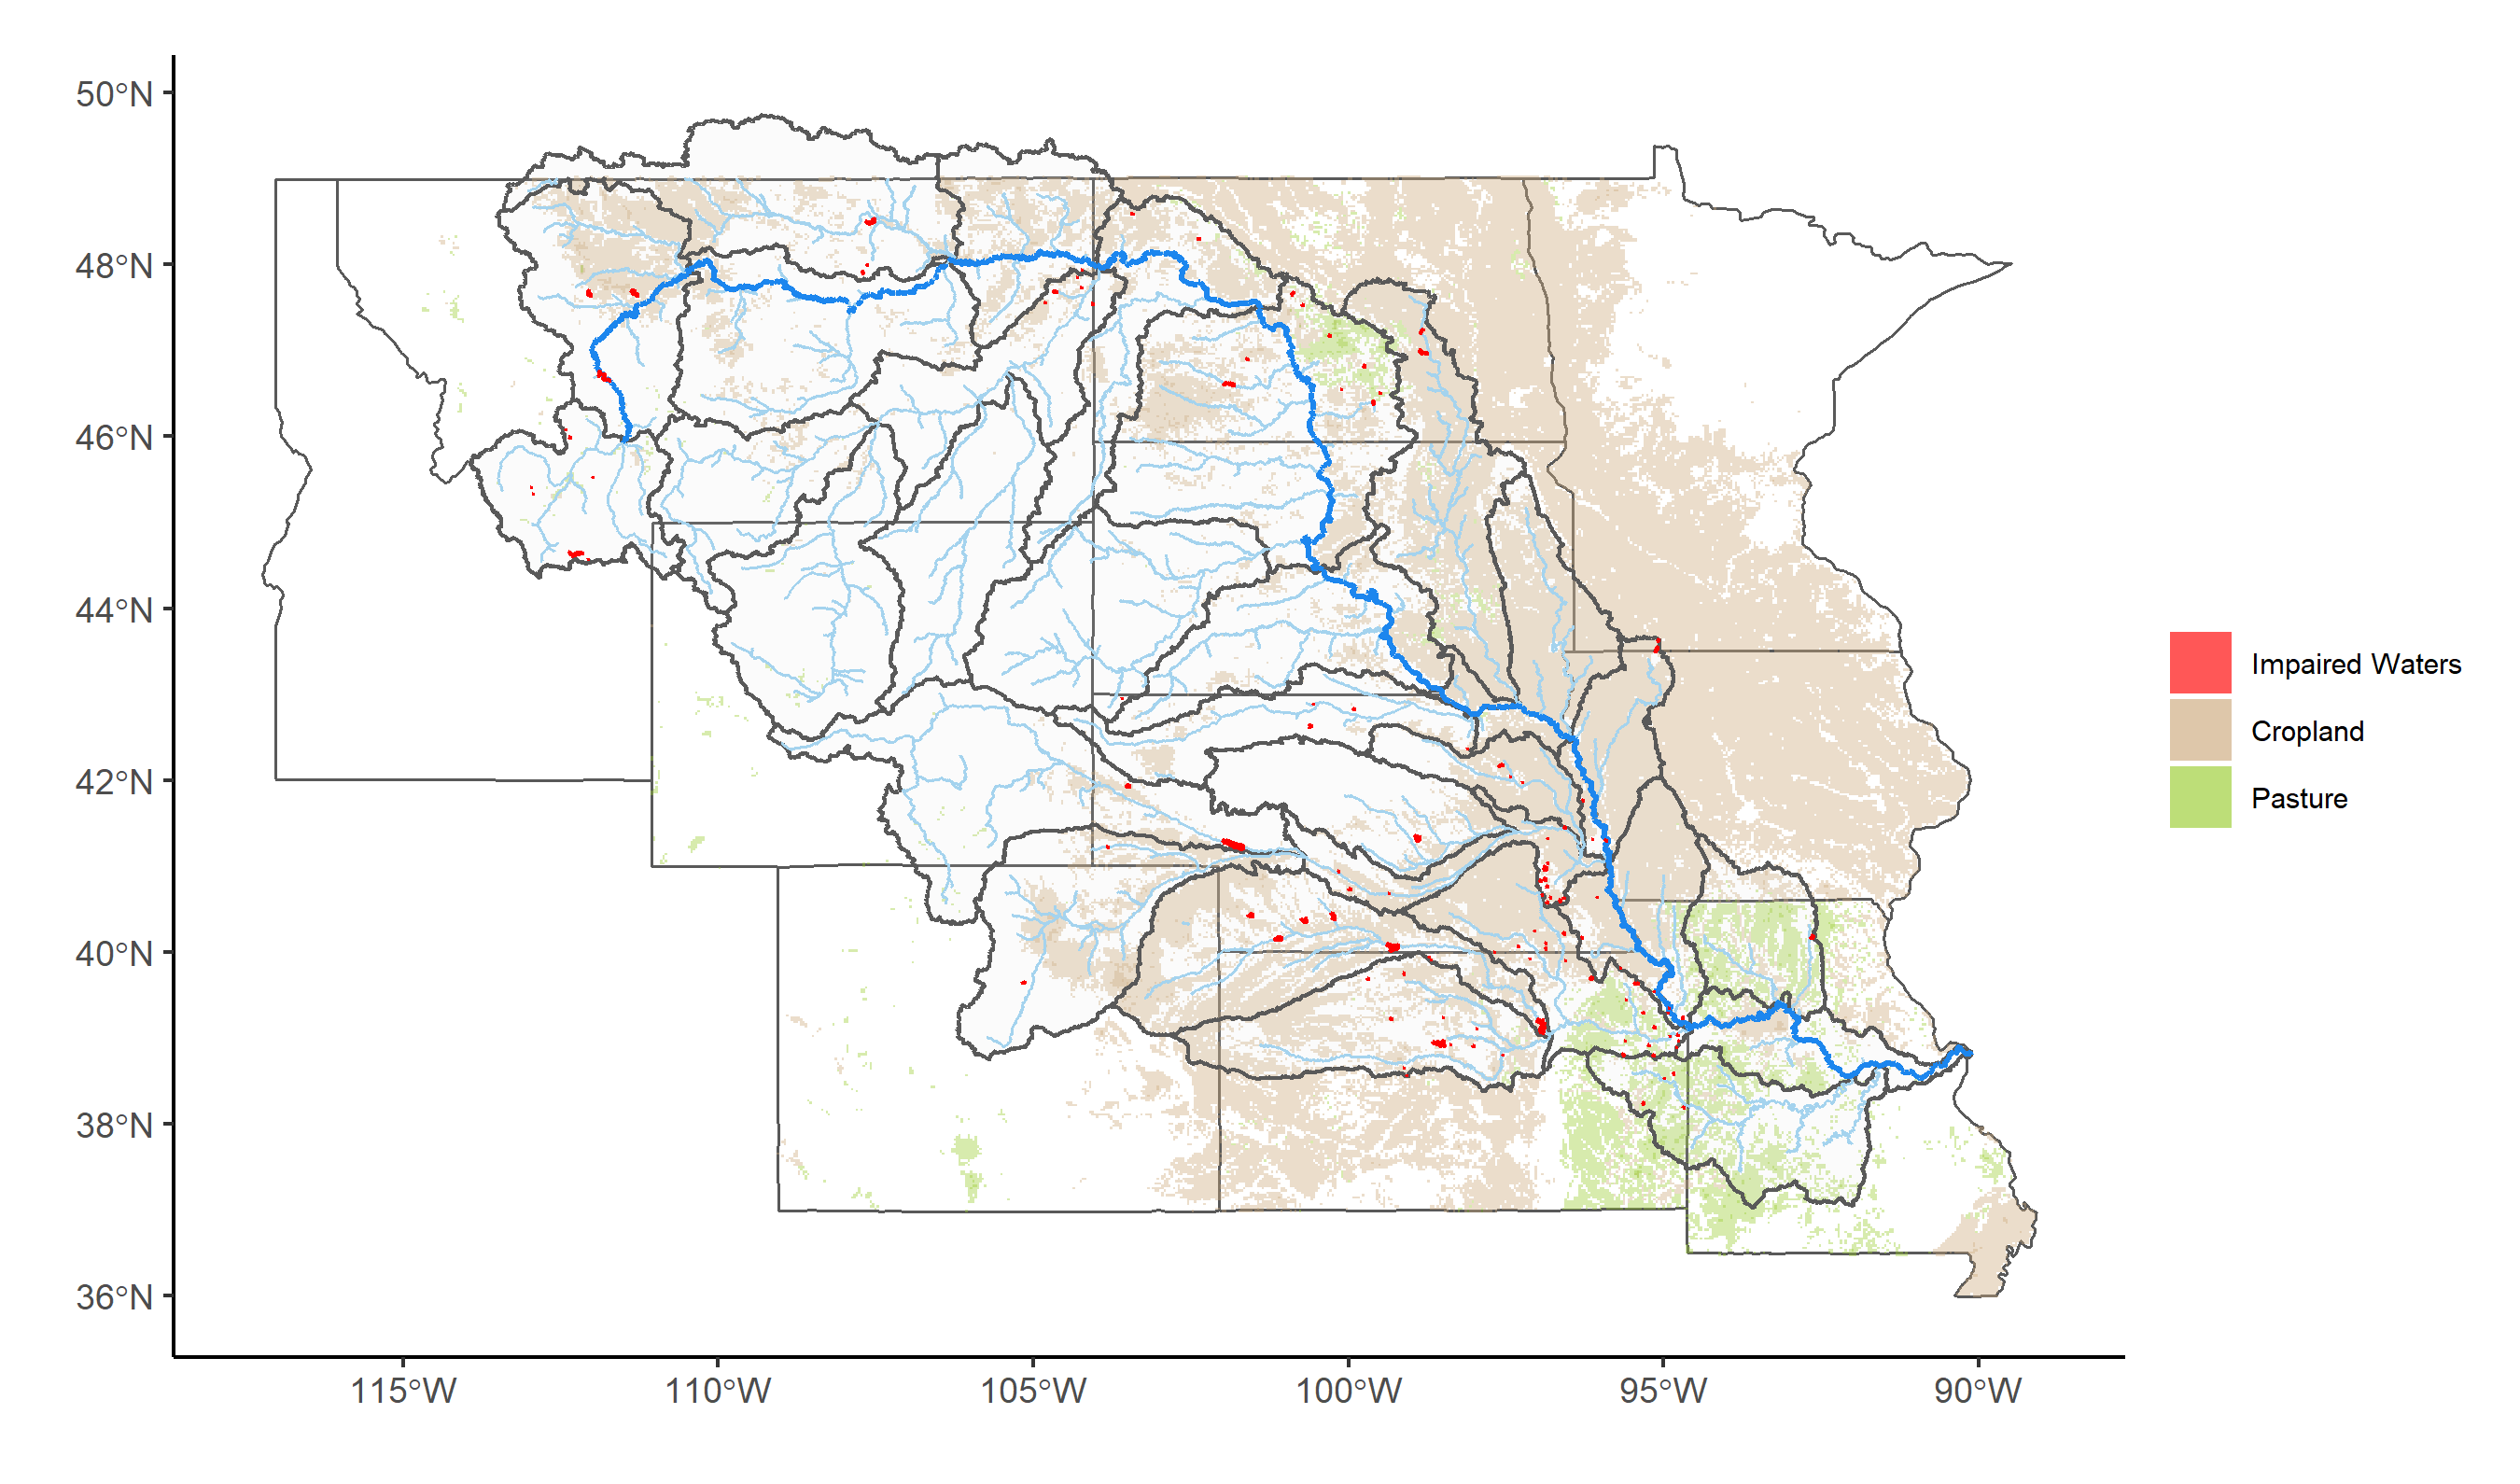
\includegraphics[width=\maxwidth]{../Figures/cropland3} \caption{\label{fig:cropland} Map of agricultural lands and impaired waters in the Missouri River Basin. Row and Close Grain Crop Cultural Formation shown by tan-colored areas, pasture and hay field shown by yellowgreen areas, imparied water bodies according to Clean Water Act Section 303(d) (EPA 2015) denoted by red areas, and all HUC4 watersheds in the Missouri River Basin (1001-1030) delineated by gray polygons. The thin light-blue lines outline all streams of a Strahler order higher than 2, and the thick blue line represents the mainstem of Missouri River.}\label{fig:cropland}
\end{figure}

Our research questions and acccompanying hypotheses are below.

\begin{enumerate}
\def\labelenumi{\arabic{enumi}.}
\item
  How have changes in discharge (i.e.~water quantity) interacted with
  nutrient enrichment (i.e.~water quality) in the Missouri River Basin?

  \begin{enumerate}
  \def\labelenumii{\alph{enumii})}
  \tightlist
  \item
    Nutrient levels have increased over time - Keqi
  \item
    Discharge has become more variable over time - Hubert
  \item
    Nutrient levels increase with discharge - Rachel
  \end{enumerate}
\item
  What effects do specific flood and drought events have on the water
  quality and quantity of rivers in the Missouri River Basin areas of
  interest?

  \begin{enumerate}
  \def\labelenumii{\alph{enumii})}
  \tightlist
  \item
    Rivers will exhibit a flushing behavior due to the land use and type
    of flow during storms - Rachel
  \item
    Discharge will decrease during drought due to decreased overland
    flow. - Caroline
  \end{enumerate}
\item
  What factors contribute to the variability of total nitrogen in the
  rivers?

  \begin{enumerate}
  \def\labelenumii{\alph{enumii})}
  \tightlist
  \item
    Land use, year, discharge, phosphorus, and HUC region will
    contribute to the variability of total nitrogen across sites -
    Rachel
  \end{enumerate}
\item
  Given past and current data, what can we predict about the future
  state of water in the Missouri River Basin?

  \begin{enumerate}
  \def\labelenumii{\alph{enumii})}
  \tightlist
  \item
    Total flow in the Missouri River Basin is decreasing
    (non-stationary) over time - Keqi
  \item
    The future situation of the river basin will see the continuation of
    current trends of decreasing overall volume of flow. - Keqi
  \end{enumerate}
\end{enumerate}

\newpage

\hypertarget{dataset-information}{%
\section{Dataset Information}\label{dataset-information}}

The data we are analyzing comes from the United States Geological Survey
(USGS) database called the National Water Information System interface,
or NWIS. We pulled data from the interface using the R package
\texttt{dataRetrieval}. Because we are interested in the lower Missouri
River basin, we pulled sites from each HUC4 subbasin from 1020 to 1030.
We chose these subbasins because they had a variety of tributaries that
all flowed into the Missouri River, representing a variety of river
sizes and lengths. We filtered these subbasin queries to only show us
sites that contained discharge, nitrogen, and phosphorus data. Once we
found the sites with all of this data, we chose 2 sites from each HUC
sub basin for a total of 22. We chose the two sites from each HUC sub
basin by comparing the periods of records for each of our chosen
variables and finding the sites with the longest periods of records. We
chose to look at two sites per HUC region (for a total of 22) in order
to maintain a digestable scope. We retrieved data on water quantity,
water quality (N, P concentrations) (Table 1).

Only seven sites within our HUC subbasin boundary contained any high
frequency nitrogen data. Therefore, we also looked at these 6 sites in
order to do analyses and answer our research question about flooding.
Since flooding and droughts can be thought of as opposites, we looked at
the same 6 sites for droughts as we did for flooding (Table 2).

We have two main datasets:

\begin{itemize}
\item
  The daily values dataset containing discharge, nitrogen, and
  phosphorus data for 22 sites.
\item
  The high freqency dataset containing high frequency data for nitrogen
  and discharge for 6 sites.
\end{itemize}

\begin{longtable}[]{@{}lcl@{}}
\toprule
Variable & Unit & Number of Sites\tabularnewline
\midrule
\endhead
Discharge & cfs or \(m^{3}\)/s & 22\tabularnewline
Time & UTC & 22\tabularnewline
Nitrogen & mg/L & 22 daily values, 6 high frequency\tabularnewline
Phosphorus & mg/L & 22\tabularnewline
\bottomrule
\end{longtable}

\textless{}Add a table that summarizes your data structure (variables,
units, ranges and/or central tendencies, data source if multiple are
used, etc.). This table can be made in markdown text or inserted as a
\texttt{kable} function in an R chunk. If the latter, do not include the
code used to generate your table.\textgreater{}

\begin{figure}[H]
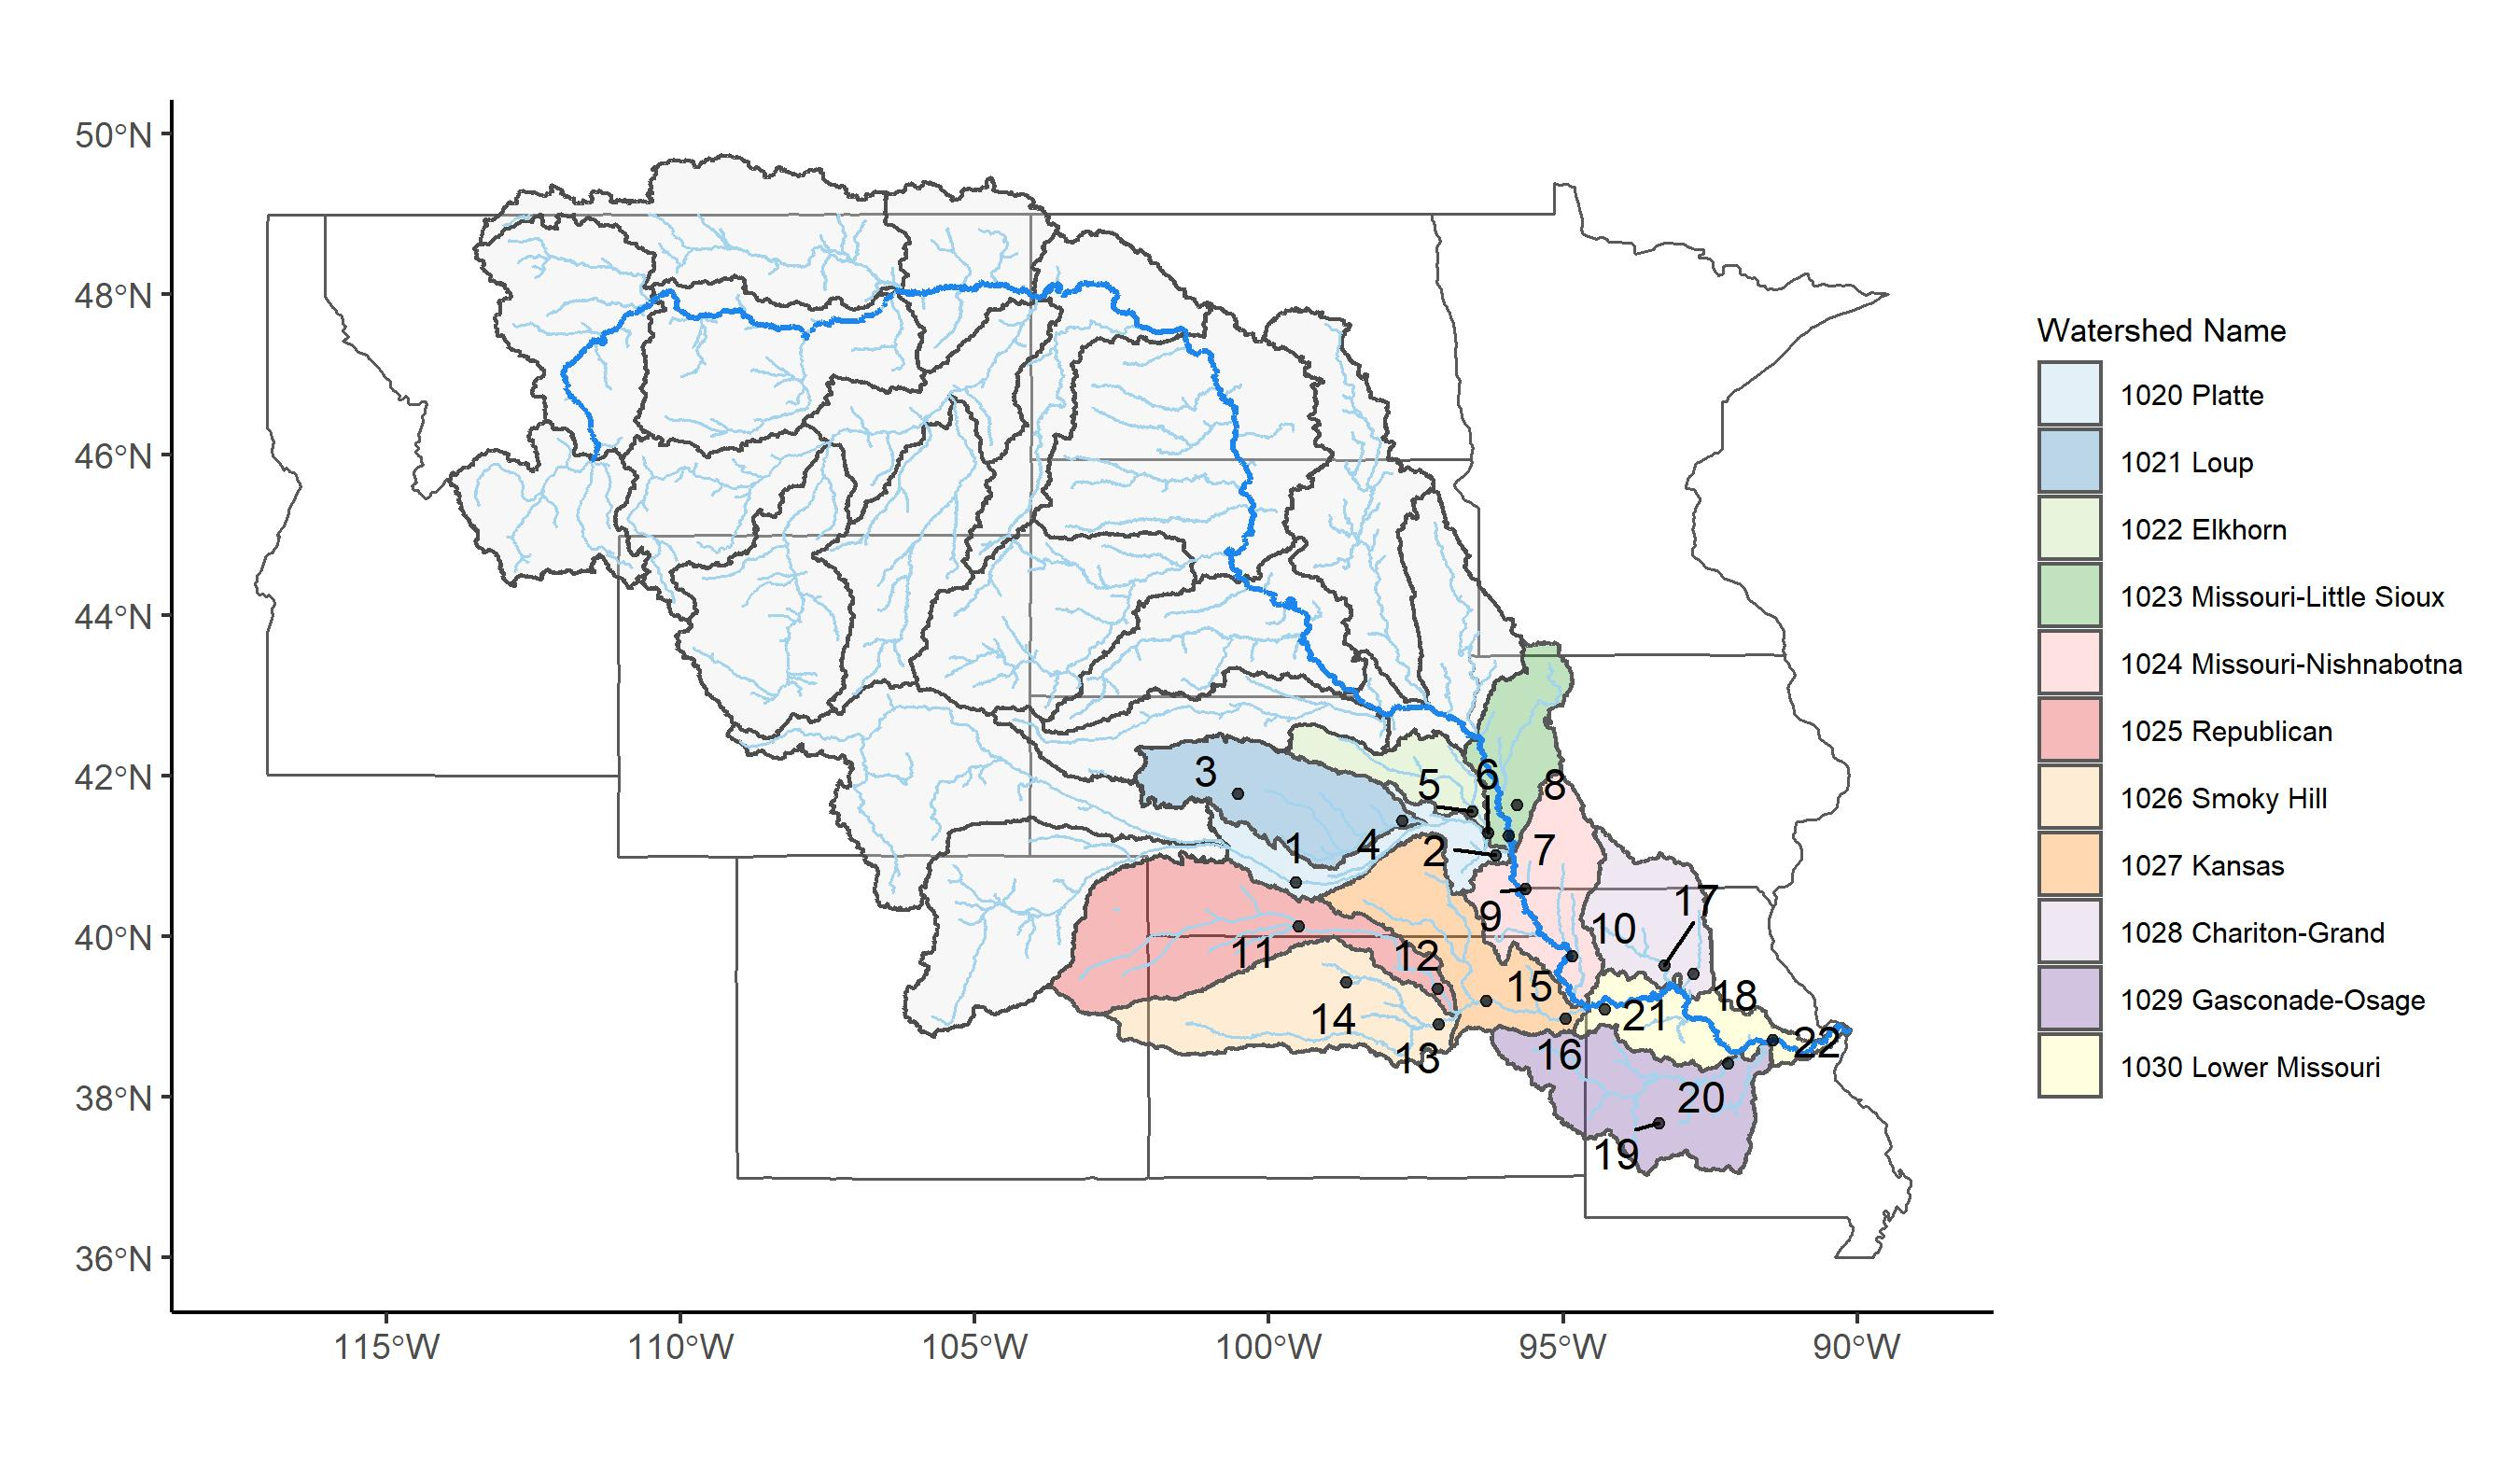
\includegraphics[width=\maxwidth]{../Figures/site_map} \caption{\label{fig:sitemap} Map of USGS sites used for long term analysis.}\label{fig:sitemap}
\end{figure}

\newpage

\hypertarget{exploratory-analysis}{%
\section{Exploratory Analysis}\label{exploratory-analysis}}

\hypertarget{exploration-of-variables}{%
\subsection{Exploration of variables}\label{exploration-of-variables}}

Basic data wrangling was needed in order to obtain all variables of
interest. After obtaining all pertinent data, each variable was
visualized in order to see the shape of the data and the range of values
(\autoref{fig:Nhist}). Any necessary transformation or cleaning was
completed after this step.

\begin{figure}[H]
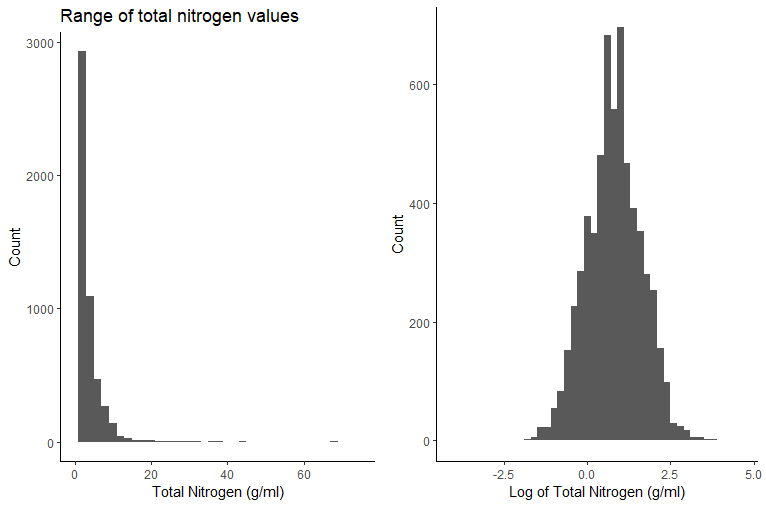
\includegraphics[width=\maxwidth]{../Figures/Nitrogenhist} \caption{\label{fig:Nhist} Histograms showing the range of total nitrogen values obtained from all sites during the total period of record. Raw (left) and logged (right) nitrogen data are shown to show that any analysis requiring normally distributed data will use the log transformed nitrogen data.}\label{fig:Nhist}
\end{figure}

Discharge, nitrogen, and phosphorus were plotted for each site and
examined together in order to see if there were any obvious patterns or
trends (\autoref{fig:dataexample}).

\begin{figure}[H]
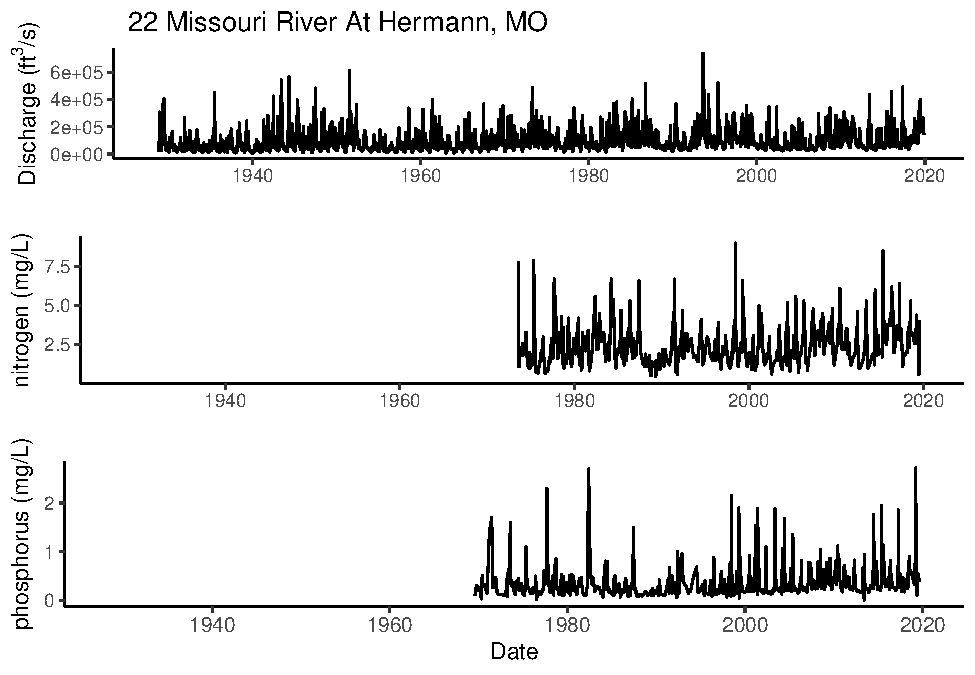
\includegraphics[width=\maxwidth]{Missouri-Reasearch-Project---FINAL_files/figure-latex/dataexample-1} \caption{\label{fig:dataexample} Discharge, Nitrogen, Phosphorus daily data of site No. 22 Missouri River At Hermann, MO.}\label{fig:dataexample}
\end{figure}

\hypertarget{yearly-discharge-pattern}{%
\subsection{Yearly Discharge Pattern}\label{yearly-discharge-pattern}}

Typical discharge patterns within a year for each HUC4 watershed from
1020 to 1030 were generated by compiling all available discharge data at
the 22 selected USGS site (\autoref{fig:dispattern}). Generally,
discharge reaches its peak during the summer and falls to minima during
the winter, and most of the sites exhibit rather high variations across
years, as indicated by the large difference between the medians and the
first or the third quartiles. Furthermore, highest variations in
discharge appear to occur in the summer, whereas discharge in the winter
varies less among years. The large variability within a year and the
seasonal pattern is only obvious in larger streams and rivers but not in
small creeks (e.g.~site 5 Maple Creek near Nickerson, site 8 Boyer
River, site 21 Small Blue River). Exceptions to the generalization are
three sites with medium discharge (site 1 Platte River, NE; site 3
Dismal River, NE; site 11 Republican River, NE). They have fairly
constant discharge and variation across years, and the the first and the
third even have slightly lower discharge during the summer. Platte River
forms by the confluence of North Platte and South Platte Rivers, and
both two have snowmelt as their water source, resulting in the observed
higher discharge during the spring and low in the summer. Dismal River
forms by two forks that arise from groundwater (Ogallala Aquifer), which
is supposed to be more stable than precipitation. The majority of
Republican River basin is underlain by Ogallala Aquifer (Reclamation
2016a), and a plausible high proportion of water source from groundwater
could explain the little variation across years.

\begin{figure}[H]
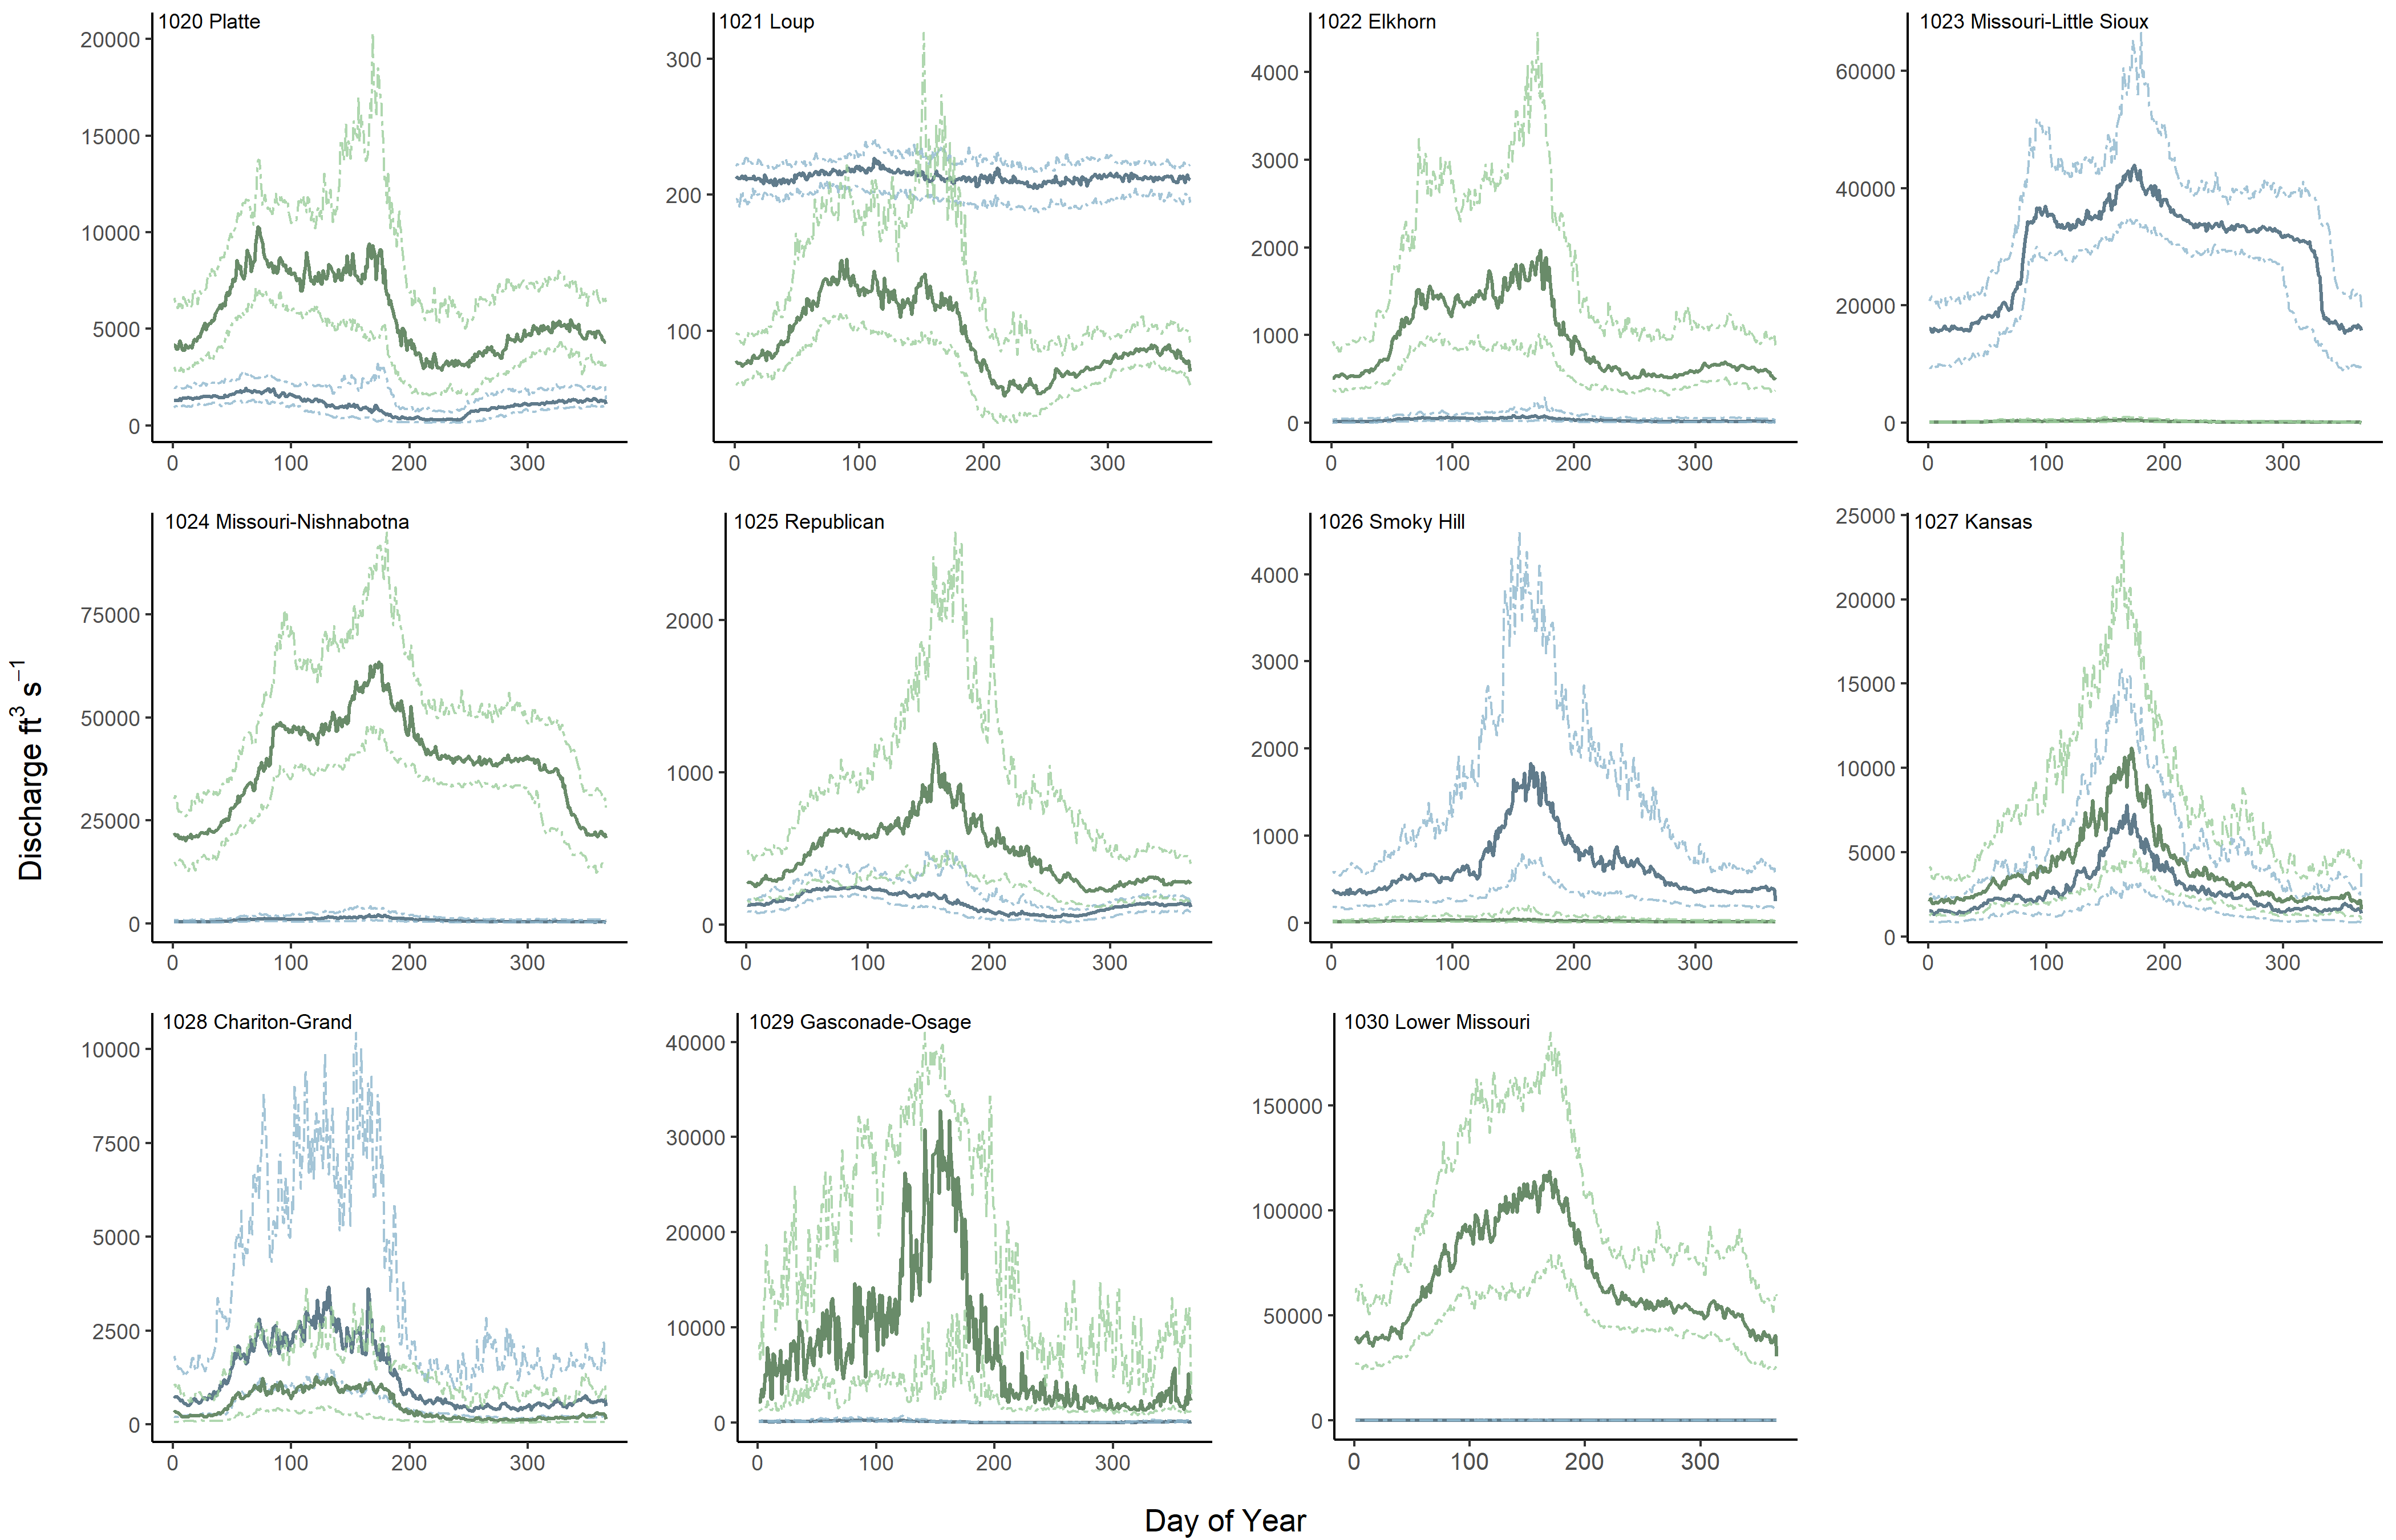
\includegraphics[width=\maxwidth]{../Figures/discharge} \caption{\label{fig:dispattern}Yearly discharge pattern for the lower Missouri HUC4 watersheds. Thick, dark lines are the median of all discharge records on a day of year, while light, thin lines are the 25th and 75 discharge quantiles on that day. The blue lines represent the first site in a HUC4 watershed, while the green lines represent the second site.}\label{fig:dispattern}
\end{figure}

\hypertarget{change-in-discharge-variations-over-years}{%
\subsection{Change in Discharge Variations over
Years}\label{change-in-discharge-variations-over-years}}

To reveal how variability of discharge has changed over time, we
analyzed the relationship between standard deviation of discharge within
a year and years, using linear models (\autoref{fig:varfig};
\autoref{tab:vartab}). Among all the 22 sites, 14 sites suggest
increasing SD over time, and 4 of them show statistically significant
increase. By contrast, only 8 sites suggest declining SD trends, and 2
of them exhibit statistically significant rising in SD. Despite that
only data from six sites (around 27\%) yield conclusive results, within
these sites the number of streams that have become more variable are two
times as many as those with decreasing variability. Thus, our results
suggest that the whole Missouri Basin appear to have become more
variable over years since around the mid-19th century. The low
percentage of significant results could result from the small effect
size, and/or the short time span of available data for some sites.
Hence, more monitoring on discharge in the basin are required in the
future to reach a more definitive conclusion.

\begin{figure}[H]
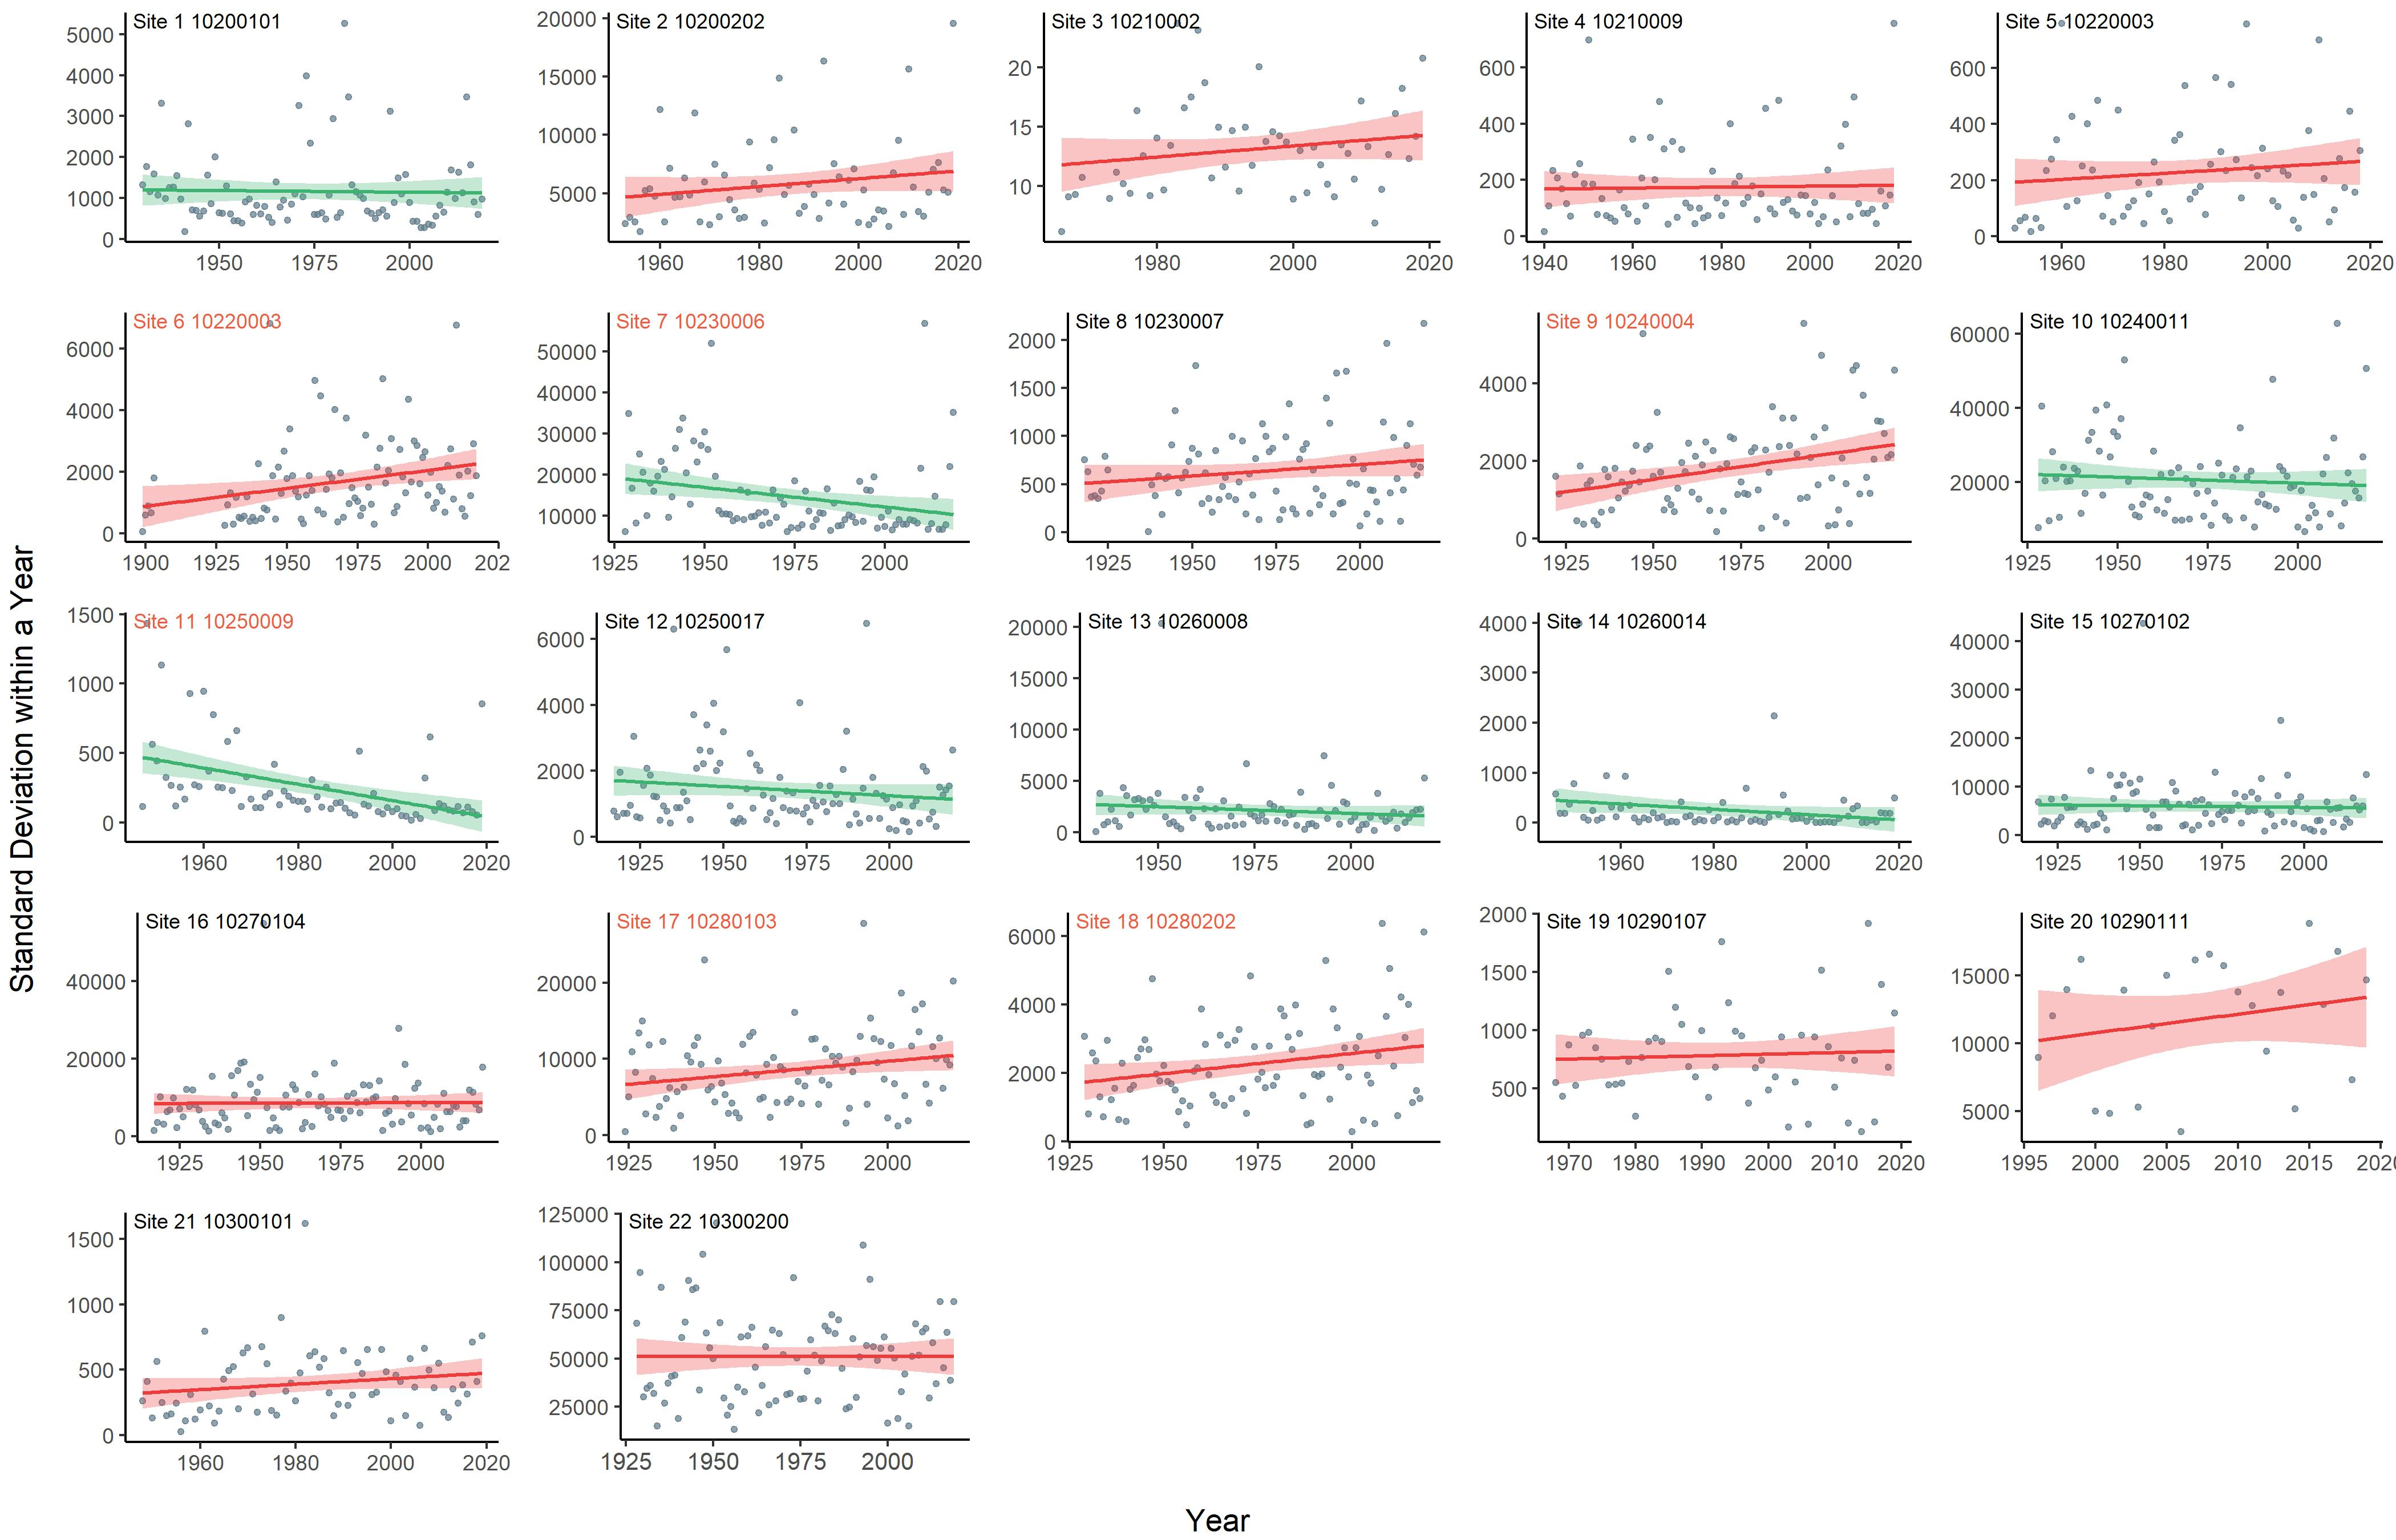
\includegraphics[width=\maxwidth]{../Figures/sd_year} \caption{\label{fig:varfig} Changes in the standard deviations (SD) of discharge within a year at 22 sites over the whole time span of available data. Red regression lines and confidence intervals suggest increasing SD, whereas blue for decreasing SD over time. Bolded site labels and HUC8, and colors with higher saturation indicate statistically significant results ($\alpha = 0.05$).}\label{fig:varfig}
\end{figure}

\begin{longtable}[]{@{}rcccc@{}}
\caption{\label{tab:vartab} Slopes of linear regression between year and
standard deviation of discharge at 22 sites.}\tabularnewline
\toprule
~ & Site Name & HUC4 & \(\beta_1\) & \emph{P}\tabularnewline
\midrule
\endfirsthead
\toprule
~ & Site Name & HUC4 & \(\beta_1\) & \emph{P}\tabularnewline
\midrule
\endhead
1 & Platte River Near Overton, NE & 1020 & -0.805 & 0.83\tabularnewline
2 & Platte River At Louisville, NE & 1020 & 33.7 & 0.144\tabularnewline
3 & Dismal River Near Thedford, NE & 1021 & 0.047 & 0.196\tabularnewline
4 & Beaver Creek At Genoa, NE & 1021 & 0.168 & 0.812\tabularnewline
5 & Maple Creek Near Nickerson, NE & 1022 & 1.1 & 0.314\tabularnewline
\textbf{6} & \textbf{Elkhorn River At Waterloo, NE} & \textbf{1022} &
\textbf{11.7} & \textbf{0.009}\tabularnewline
\textbf{7} & \textbf{Missouri River At Omaha, NE} & \textbf{1023} &
\textbf{-95.2} & \textbf{0.0093}\tabularnewline
8 & Boyer River At Logan, IA & 1023 & 2.4 & 0.134\tabularnewline
\textbf{9} & \textbf{Nishnabotna River Above Hamburg, IA} &
\textbf{1024} & \textbf{13} & \textbf{0.0018}\tabularnewline
10 & Missouri River At St.~Joseph, MO & 1024 & -32.1 &
0.452\tabularnewline
\textbf{11} & \textbf{Republican River Near Orleans, NE} & \textbf{1025}
& \textbf{-5.86} & \textbf{1e-04}\tabularnewline
12 & Republican R At Clay Center, KS & 1025 & -5.58 &
0.157\tabularnewline
13 & Smoky Hill R At Enterprise, KS & 1026 & -12.9 &
0.226\tabularnewline
14 & Sf Solomon R At Osborne, KS & 1026 & -5.27 & 0.0716\tabularnewline
15 & Kansas R At Wamego, KS & 1027 & -6.68 & 0.714\tabularnewline
16 & Kansas R At Desoto, KS & 1027 & 2.56 & 0.91\tabularnewline
\textbf{17} & \textbf{Grand River Near Sumner, MO} & \textbf{1028} &
\textbf{40.4} & \textbf{0.0264}\tabularnewline
\textbf{18} & \textbf{Chariton River Near Prairie Hill, MO} &
\textbf{1028} & \textbf{11.9} & \textbf{0.0199}\tabularnewline
19 & Pomme De Terre River Near Polk, MO & 1029 & 1.39 &
0.704\tabularnewline
20 & Osage River Below St.~Thomas, MO & 1029 & 138 &
0.311\tabularnewline
21 & Little Blue River Near Lake City, MO & 1030 & 2.1 &
0.141\tabularnewline
22 & Missouri River At Hermann, MO & 1030 & 0.657 & 0.994\tabularnewline
\bottomrule
\end{longtable}

\hypertarget{analysis}{%
\section{Analysis}\label{analysis}}

\textless{}Insert visualizations and text describing your main analyses.
Format your R chunks so that graphs are displayed but code and other
output is not displayed. Instead, describe the results of any
statistical tests in the main text (e.g., ``Variable x was significantly
different among y groups (ANOVA; df = 300, F = 5.55, p \textless{}
0.0001)''). Each paragraph, accompanied by one or more visualizations,
should describe the major findings and how they relate to the question
and hypotheses. Divide this section into subsections, one for each
research question.\textgreater{}

\textless{}Each figure should be accompanied by a caption, and each
figure should be referenced within the text\textgreater{}

\hypertarget{question-1-how-have-changes-in-discharge-interacted-with-nutrient-enrichment-in-the-missouri-river-basin}{%
\subsection{Question 1: How have changes in discharge interacted with
nutrient enrichment in the Missouri River
Basin?}\label{question-1-how-have-changes-in-discharge-interacted-with-nutrient-enrichment-in-the-missouri-river-basin}}

In order to determine whether nutrient levels increase with discharge,
C-Q (concentration - discharge) plots were created for each site
(\autoref{fig:CQplot}). At sites with high frequency nitrogen data, high
frequency nitrogen and discharge values were used. When sites did not
have high frequency nitrogen data, daily values were used. The 22 sites
showed no consistent pattern when it came to nitrogen and discharge.

\begin{figure}[H]
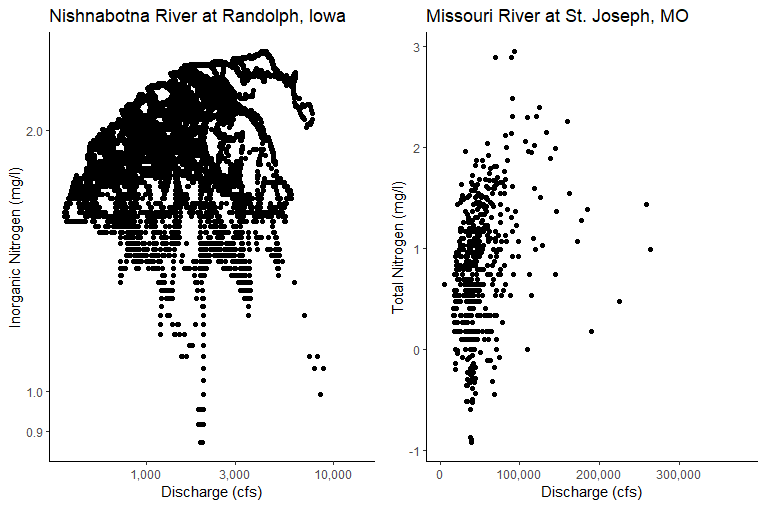
\includegraphics[width=\maxwidth]{../Figures/CQplots} \caption{\label{fig:CQplot} C-Q plots of two sites in the Missouri River Basin. High frequency (left) and daily values (right) shown for two different sites. Nitrogen values are log transformed.}\label{fig:CQplot}
\end{figure}

\hypertarget{question-2-what-effects-do-specific-flood-and-drought-events-have-on-the-water-quality-and-quantity-of-rivers-in-the-missouri-river-basin-areas-of-interest}{%
\subsection{Question 2: What effects do specific flood and drought
events have on the water quality and quantity of rivers in the Missouri
River Basin areas of
interest?}\label{question-2-what-effects-do-specific-flood-and-drought-events-have-on-the-water-quality-and-quantity-of-rivers-in-the-missouri-river-basin-areas-of-interest}}

\hypertarget{flooding}{%
\subsubsection{Flooding}\label{flooding}}

Population of each county (from the 2010 census) in the four states that
make up our region area of interest (Kansas, Nebraska, Missouri, and
Iowa) were found using the ``counties'' database from R's
\texttt{noncensus} package. We decided that population could be used as
a proxy for land cover, as a greater population would indicate more
development and fewer agricultural fields or open spaces.

Baseflow and quickflow from each site were determined with the
\texttt{EcoHydRology} package. After linearly interpolating the
instantaneous discharge data in order to account for gaps, total
baseflow volume was found and the percent of discharge exported as
baseflow was calculated. We predicted that a site within a county with a
large population would have a lower percent of its discharge exported as
baseflow, because quickflow would be more common in areas with a lot of
development. Similarly, we also predicted that a site within a county
with a small population would have a greater percentage of its discharge
coming from baseflow. More developed areas often have flashier floods,
and so we were curious to see whether we can relate population to an
element of flashiness - the percentage of discharge exported as
quickflow.

Contrary to our hypotheses, greater county population does not
contribute to a decrease in percent of discharge as baseflow (p =
0.4199, F = 0.8067) in our sites of interest. This may be due to our
small sample size of sites, or perhaps the size of the rivers in our
study.

High frequency nitrogen data was only available for seven sites within
our region. In order to better understand the behavior of rivers during
floods, we examined dygraph plots of discharge and nitrogen, and created
hysteresis plots. Storms from the fall of 2018 (September - December)
were examined for each river site with data from that time period. We
chose to only look at storms that occurred in the second half of the
year in order to avoid conflating snowpack melt and precipitation
affects.

We predicted that most rivers in the area would behave the same way, and
that rivers would exhibit flushing behavior. We thought that flushing
rivers would be more prevalent because of the many agricultural fields
in our region of study, and any overland flow to the rivers would bring
with it a high concentration of nutrients (nitrogen being one of them)
from the fertilized fields. Our results say otherwise (Table 2). Our
sites of interest had both positive and negative slopes in the
hysteresis plots, and also exhibited both clockwise and counter
clockwise directions of flow (\autoref{fig:RandolphStorm}). The same
river was analyzed multiple times throughout the year, and even the same
river showed different slopes and directions in the hysteresis plots for
different storm events.

\begin{longtable}[]{@{}lclll@{}}
\toprule
\begin{minipage}[b]{0.15\columnwidth}\raggedright
Site Name\strut
\end{minipage} & \begin{minipage}[b]{0.22\columnwidth}\centering
Site Number\strut
\end{minipage} & \begin{minipage}[b]{0.20\columnwidth}\raggedright
Time Period\strut
\end{minipage} & \begin{minipage}[b]{0.17\columnwidth}\raggedright
Direction\strut
\end{minipage} & \begin{minipage}[b]{0.12\columnwidth}\raggedright
Slope\strut
\end{minipage}\tabularnewline
\midrule
\endhead
\begin{minipage}[t]{0.15\columnwidth}\raggedright
West Nishnabotna River in Randolph, IA\strut
\end{minipage} & \begin{minipage}[t]{0.22\columnwidth}\centering
06808500\strut
\end{minipage} & \begin{minipage}[t]{0.20\columnwidth}\raggedright
Oct 7 - 13, 2018\strut
\end{minipage} & \begin{minipage}[t]{0.17\columnwidth}\raggedright
counter clockwise\strut
\end{minipage} & \begin{minipage}[t]{0.12\columnwidth}\raggedright
negative (Figure xx)\strut
\end{minipage}\tabularnewline
\begin{minipage}[t]{0.15\columnwidth}\raggedright
Nodaway River at Clarinda, IA\strut
\end{minipage} & \begin{minipage}[t]{0.22\columnwidth}\centering
06817000\strut
\end{minipage} & \begin{minipage}[t]{0.20\columnwidth}\raggedright
Oct 8 - 12, 2018\strut
\end{minipage} & \begin{minipage}[t]{0.17\columnwidth}\raggedright
clockwise\strut
\end{minipage} & \begin{minipage}[t]{0.12\columnwidth}\raggedright
negative\strut
\end{minipage}\tabularnewline
\begin{minipage}[t]{0.15\columnwidth}\raggedright
Kansas River in Desoto, KS\strut
\end{minipage} & \begin{minipage}[t]{0.22\columnwidth}\centering
06892350\strut
\end{minipage} & \begin{minipage}[t]{0.20\columnwidth}\raggedright
Nov 30 - Dec 5, 2018\strut
\end{minipage} & \begin{minipage}[t]{0.17\columnwidth}\raggedright
counter clockwise\strut
\end{minipage} & \begin{minipage}[t]{0.12\columnwidth}\raggedright
positive\strut
\end{minipage}\tabularnewline
\begin{minipage}[t]{0.15\columnwidth}\raggedright
Missouri River at Hermann, MO\strut
\end{minipage} & \begin{minipage}[t]{0.22\columnwidth}\centering
06934500\strut
\end{minipage} & \begin{minipage}[t]{0.20\columnwidth}\raggedright
Oct 7 - 20, 2018\strut
\end{minipage} & \begin{minipage}[t]{0.17\columnwidth}\raggedright
counter clockwise\strut
\end{minipage} & \begin{minipage}[t]{0.12\columnwidth}\raggedright
negative\strut
\end{minipage}\tabularnewline
\begin{minipage}[t]{0.15\columnwidth}\raggedright
Mill C at Johnson Drive, Shawnee, KS\strut
\end{minipage} & \begin{minipage}[t]{0.22\columnwidth}\centering
06892513\strut
\end{minipage} & \begin{minipage}[t]{0.20\columnwidth}\raggedright
Nov 27 - Dec 4, 2018\strut
\end{minipage} & \begin{minipage}[t]{0.17\columnwidth}\raggedright
clockwise\strut
\end{minipage} & \begin{minipage}[t]{0.12\columnwidth}\raggedright
negative\strut
\end{minipage}\tabularnewline
\begin{minipage}[t]{0.15\columnwidth}\raggedright
Grand River, Sumner MO\strut
\end{minipage} & \begin{minipage}[t]{0.22\columnwidth}\centering
06902000\strut
\end{minipage} & \begin{minipage}[t]{0.20\columnwidth}\raggedright
Sep 6 - 10, 2018\strut
\end{minipage} & \begin{minipage}[t]{0.17\columnwidth}\raggedright
clockwise\strut
\end{minipage} & \begin{minipage}[t]{0.12\columnwidth}\raggedright
positive\strut
\end{minipage}\tabularnewline
\bottomrule
\end{longtable}

\begin{figure}
\centering
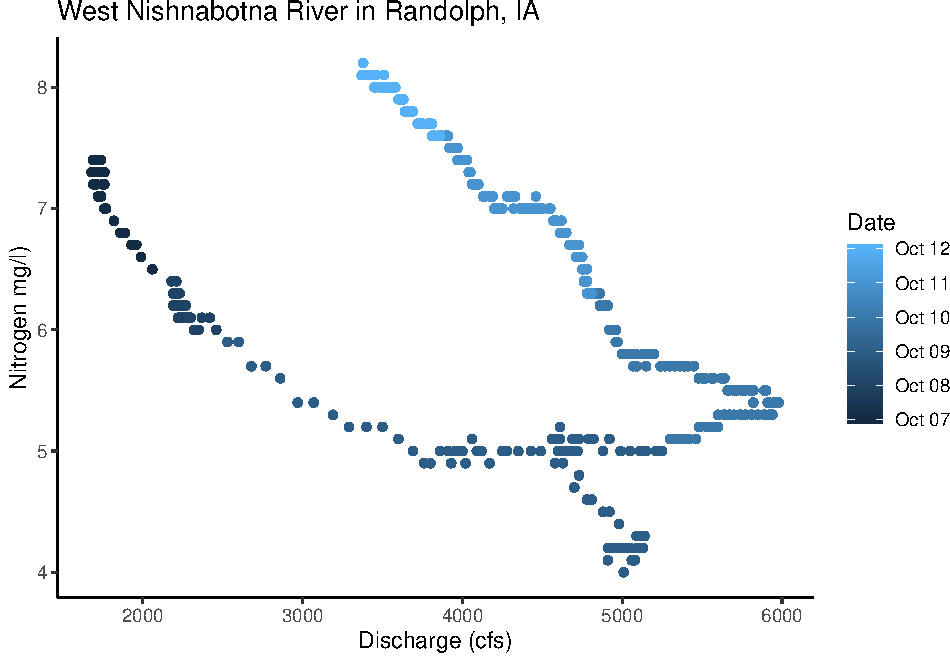
\includegraphics{Missouri-Reasearch-Project---FINAL_files/figure-latex/Randolphstorm-1.pdf}
\caption{Hyteresis plot for site in Randolph, IA that shows a negative
slope (diluting behavior) in a counter clockwise direction.}
\end{figure}

\hypertarget{question-3-what-factors-contribute-to-the-variability-of-total-nitrogen-in-the-rivers}{%
\subsection{Question 3: What factors contribute to the variability of
total nitrogen in the
rivers?}\label{question-3-what-factors-contribute-to-the-variability-of-total-nitrogen-in-the-rivers}}

\hypertarget{question-4-given-past-and-current-data-what-can-we-predict-about-the-future-state-of-water-in-the-missouri-river-basin}{%
\subsection{Question 4: Given past and current data, what can we predict
about the future state of water in the Missouri River
Basin?}\label{question-4-given-past-and-current-data-what-can-we-predict-about-the-future-state-of-water-in-the-missouri-river-basin}}

\begin{longtable}[]{@{}llllllllllllll@{}}
\toprule
\begin{minipage}[b]{0.05\columnwidth}\raggedright
Site Name\strut
\end{minipage} & \begin{minipage}[b]{0.06\columnwidth}\raggedright
Site Number\strut
\end{minipage} & \begin{minipage}[b]{0.05\columnwidth}\raggedright
Dec.~2019\strut
\end{minipage} & \begin{minipage}[b]{0.04\columnwidth}\raggedright
Jan.~2020\strut
\end{minipage} & \begin{minipage}[b]{0.05\columnwidth}\raggedright
Feb.~2020\strut
\end{minipage} & \begin{minipage}[b]{0.05\columnwidth}\raggedright
Mar.~2020\strut
\end{minipage} & \begin{minipage}[b]{0.05\columnwidth}\raggedright
Apr.~2020\strut
\end{minipage} & \begin{minipage}[b]{0.04\columnwidth}\raggedright
May 2020\strut
\end{minipage} & \begin{minipage}[b]{0.05\columnwidth}\raggedright
June 2020\strut
\end{minipage} & \begin{minipage}[b]{0.05\columnwidth}\raggedright
July 2020\strut
\end{minipage} & \begin{minipage}[b]{0.05\columnwidth}\raggedright
Aug.~2020\strut
\end{minipage} & \begin{minipage}[b]{0.05\columnwidth}\raggedright
Sept.~2020\strut
\end{minipage} & \begin{minipage}[b]{0.04\columnwidth}\raggedright
Oct.~2020\strut
\end{minipage} & \begin{minipage}[b]{0.04\columnwidth}\raggedright
Nov.~2020\strut
\end{minipage}\tabularnewline
\midrule
\endhead
\bottomrule
\end{longtable}

Platte River near Overton, Nebr. Platte River at Louisville, Nebr.
Dismal River near Thedford, Nebr. Beaver Creek at Genoa, Nebr. Maple
Creek near Nickerson, Nebr. Elkhorn River at Waterloo, Nebr. Missouri
River at Omaha, NE Boyer River at Logan, IA Nishnabotna River above
Hamburg, IA Missouri River at St.~Joseph, MO Republican River near
Orleans, Nebr. REPUBLICAN R AT CLAY CENTER, KS SMOKY HILL R AT
ENTERPRISE, KS SF SOLOMON R AT OSBORNE, KS KANSAS R AT WAMEGO, KS KANSAS
R AT DESOTO, KS Grand River near Sumner, MO Chariton River near Prairie
Hill, MO Pomme de Terre River near Polk, MO Osage River below
St.~Thomas, MO Little Blue River near Lake City, MO Missouri River at
Hermann, MO

\hypertarget{droughts}{%
\subsubsection{Droughts}\label{droughts}}

Droughts in the Missouri River Basin were known to occur throughout the
years.

Table summarizing the 7Q10 values for each of the streams that were
analyzed for droughts.

\begin{longtable}[]{@{}lll@{}}
\toprule
Site Name & Site Number & 7Q10 Minimum Discharge (cfs)\tabularnewline
\midrule
\endhead
West Nishnabotna River in Randolph, IA & 06808500 & 41.3\tabularnewline
Nodaway River at Clarinda, IA & 06817000 & 5.93\tabularnewline
Kansas River in Desoto, KS & 06892350 & 562\tabularnewline
Missouri River at Hermann, MO & 06934500 & 12414\tabularnewline
Mill C at Johnson Drive, Shawnee, KS & 06892513 & 1.47\tabularnewline
Grand River, Sumner MO & 06902000 & 39.1\tabularnewline
\bottomrule
\end{longtable}

\newpage

\hypertarget{summary-and-conclusions}{%
\section{Summary and Conclusions}\label{summary-and-conclusions}}

\textless{}Summarize your major findings from your analyses in a few
paragraphs. What conclusions do you draw from your findings? Relate your
findings back to the original research questions and
rationale.\textgreater{}

\newpage

\hypertarget{references}{%
\section*{References}\label{references}}
\addcontentsline{toc}{section}{References}

\hypertarget{refs}{}
\leavevmode\hypertarget{ref-nrc2002}{}%
Council, National Research. 2002. \emph{The Missouri River Ecosystem:
Exploring the Prospects for Recovery}. Book. Washington, DC: The
National Academies Press. \url{https://doi.org/doi:10.17226/10277}.

\leavevmode\hypertarget{ref-usace2018}{}%
Engineers Missouri River Basin Water Management Division, U.S. Army
Corps of. 2018. ``Master Water Control Manual Missouri River Basin.''
Government Document.

\leavevmode\hypertarget{ref-noaa2013}{}%
Force, NOAA Drought Task. 2013. ``An Interpretation of the Origins of
the 2012 Central Great Plains Drought.'' Government Document.
\url{https://cpo.noaa.gov/Meet-the-Divisions/Earth-System-Science-and-Modeling/MAPP/MAPP-Task-Forces/Drought/Drought-Task-Force-II/An-Interpretation-of-the-Origins-of-the-2012-Central-Great-Plains-Drought}.

\leavevmode\hypertarget{ref-kammerer1990}{}%
Kammerer, J.C. 1990. ``Largest Rivers in the United States.'' Report.
U.S. Geological Survey, Department of the Interior.

\leavevmode\hypertarget{ref-noaa2012}{}%
Oceanic, National, and Atmospheric Administration. 2012. ``Service
Assessment the Missouri/Souris River Floods of May -- August 2011.''
Government Document.

\leavevmode\hypertarget{ref-bor2016-2}{}%
Reclamation, Bureau of. 2016a. ``Republican River Basin Study.''
Government Document.
\url{https://www.usbr.gov/watersmart/bsp/docs/finalreport/republican/republican-river-basin-study-final-report.pdf}.

\leavevmode\hypertarget{ref-bor2016-1}{}%
---------. 2016b. ``SECURE Water Act Section 9503(c) Report to
Congress.'' Report.
\url{https://www.usbr.gov/climate/secure/docs/2016secure/2016SECUREReport-chapter6.pdf}.


\end{document}
